\documentclass[a4paper,11pt]{article}
\usepackage[utf8]{inputenc}
\usepackage[italian]{babel}
\usepackage{amsmath, amssymb}
\usepackage{listings}
\usepackage{color}
\usepackage{xcolor}
\usepackage{times}
\usepackage{geometry}
\usepackage{graphicx}
\usepackage{listings}
\usepackage{hyperref}
\usepackage[utf8]{inputenc}

\geometry{a4paper, margin=1in}

% Colors for code listings
\definecolor{commentgray}{gray}{0.5}
\definecolor{stringgreen}{rgb}{0,0.6,0}
\definecolor{keywordblue}{rgb}{0,0,0.6}

% Listing settings for code
\lstset{
    basicstyle=\ttfamily\small,
    keywordstyle=\color{keywordblue},
    stringstyle=\color{stringgreen},
    commentstyle=\color{commentgray}\itshape,
    breaklines=true,
    frame=none,
    numbers=none,
    numberstyle=\tiny,
    tabsize=2,
    showstringspaces=false,
    captionpos=b
}

\geometry{top=3cm, bottom=3cm, left=3cm, right=3cm}


\begin{document}

% Inserisci il logo (spazio riservato)
    \begin{center}
        
\includegraphics[width=3cm]{Immagini/logo.png}
    \end{center}

% Titolo dell'università
    \begin{center}
        \textsc{\textbf{Università degli Studi di Urbino}}\\
        \textsc{Dipartimento di Scienze Pure e Applicate}\\
        \textsc{Corso di Laurea in Informatica Applicata}
    \end{center}

    \vspace{2cm}

% Titolo del progetto
    \begin{center}
        \textbf{\Large Progetto di Programmazione Logica e Funzionale}
    \end{center}

    \vspace{2cm}

% Informazioni dello studente
    \begin{center}
        \textbf{di Giaconi Christian, Giacomo Rossi} \\ % Spazio per il nome dello studente
        \textbf{Matricola 314045, 314671} \\ % Spazio per la matricola
        \textbf{Anno di corso: terzo}
    \end{center}

    \vspace{2cm}

% Anno accademico e docente
    \begin{center}
        \textbf{Anno Accademico 2023/2024 - Sessione invernale}\\
        \vspace{1cm}
        \textbf{Docente: Prof. Marco Bernardo}
    \end{center}

    \newpage
    \tableofcontents

    \newpage
    \section{Specifica del problema}
    \textit
    {
        \noindent
        Scrivere un programma Haskell e un programma Prolog per implementare un sistema di raccomandazione
        di canzoni. Il programma legge le canzoni espresse in quattro attributi: titolo, artista,
        genere musicale e punteggio; da un file con valori separati da virgole, il cui nome viene acquisito
    da tastiera e le suggerisce all’utente basandosi sulle sue preferenze musicali, utilizzando un
    punteggio di gradimento acquisito da tastiera e configurato su uno o piu generi, per creare una
    classifica con le canzoni ordinate secondo il punteggio ponderato da quello di gradimento del o
    dei generi musicali.
    }

    \newpage
    \section{Analisi del problema}
    \subsection{Dati in ingresso}
    \begin{itemize}
        \item Un file di valori separati da virgole contenenti le canzoni nel formato:
        \begin{verbatim}
    Titolo,Artista,Genere,Punteggio
        \end{verbatim}
        \item Una lista di generi preferiti.
        \item Pesi numerici assegnati ai generi preferiti.
    \end{itemize}

    \subsection{Dati in uscita}
    \begin{itemize}
        \item Una classifica ordinata di canzoni basata sui punteggi ponderati.
        \item Una lista dei generi impostati come preferiti con il rispettivo peso associato.
    \end{itemize}

    \subsection{Relazioni intercorrenti}
    Ogni canzone è definita da quattro attributi principali:
    \begin{itemize}
        \item \textbf{Titolo}: la denominazione della canzone.
        \item \textbf{Artista}: l’autore o il gruppo musicale che l’ha prodotta.
        \item \textbf{Genere}: la categoria musicale di appartenenza (ad esempio, pop, rock, jazz).
        \item \textbf{Punteggio}: una valutazione numerica che rappresenta il grado di apprezzamento della canzone.
    \end{itemize}

    Il \textbf{Punteggio Ponderato} viene calcolato secondo la seguente formula:
    \begin{center}
        \textit{
            \[
                \text{Punteggio Ponderato} =
                \begin{cases}
                    \text{Punteggio} \times \text{Peso Genere} & \text{se il genere è preferito dall’utente} \\
                    \text{Punteggio originale} & \text{qualora non ci sia preferenza}
                \end{cases}
            \]
        }
    \end{center}

    \noindent
    Il \textbf{Peso Genere} è un coefficiente che modifica il punteggio di una canzone in base alla rilevanza attribuita dall'utente ai generi musicali di suo interesse.

    \newpage
    \section{Progettazione dell'algoritmo}
    \subsection{Scelte di progetto}
    Per via della natura dei dati gestiti dal programma, è necessario prevedere una rappresentazione che permetta una gestione flessibile ed efficace. I dati acquisiti dall'utente possono essere classificati in categorie diverse, quali stringhe, valori numerici interi e decimali.

    Considerando la varietà di questi dati, si è scelto di adottare una convenzione che garantisca la coerenza degli input. Ad esempio, i valori numerici verranno utilizzati per selezionare opzioni o pesi, mentre le stringhe saranno impiegate per identificare file o informazioni sulle canzoni presenti in esso. Si è deciso di usare la lista come struttura dati in quanto si addice ai linguaggi che verranno usati.

    Eventuali errori nell'input saranno tollerati nella misura in cui non compromettono la sintassi o la logica del programma.

    \subsection{Passi dell'algoritmo}
    I passi principali dell'algoritmo, indipendentemente dal linguaggio di implementazione, sono i seguenti:

    \begin{enumerate}
        \item \textbf{Caricare le informazioni di base:}
        Acquisire un file contenente le canzoni, comprensivo di informazioni quali titolo, artista, genere e punteggio.
        \item \textbf{Inserire le preferenze dell'utente:}
        L’utente specifica i generi musicali preferiti e i relativi pesi, che influenzeranno il calcolo della raccomandazione.
        \item \textbf{Calcolare i punteggi ponderati:}
        Per ogni canzone, viene determinato un punteggio combinando il peso associato al genere con il punteggio specifico originale della canzone.
        \item \textbf{Ordinare le canzoni:}
        Le canzoni vengono organizzate in ordine decrescente in base al punteggio ponderato, producendo una classifica ordinata.
        \item \textbf{Fornire le raccomandazioni:}
        L'algoritmo restituisce una lista ordinata delle canzoni con i relativi punteggi, permettendo all'utente di identificare facilmente le raccomandazioni più rilevanti.
    \end{enumerate}
    \newpage
    \section{Implementazione dell'algoritmo}
    \subsection{Implementazione in Haskell}
    Il file \texttt{raccomandazioni.hs} implementa l'algoritmo in Haskell. Un esempio di calcolo dei punteggi ponderati:
    \begin{lstlisting}[language=Haskell]
    -- #########################################################
-- # Corso di Programmazione Logica e Funzionale           #
-- # Progetto di raccomandazione di canzoni                #
-- # Studente: Giaconi Christian, Giacomo Rossi            #
-- # Matricola: 314045, 314671                             #
-- #########################################################

{-  Specifica: scrivere un programma Haskell per implementare un sistema di raccoandazione di canzoni.
    Il programma legge le canzoni espresse in quattro attributi: titolo, artista,
    genere musicale e punteggio; da un file con valori separati da virgole, il cui nome viene acquisito da tastiera e le suggerisce all’utente basandosi sulle sue preferenze musicali, utilizzando un
    punteggio di gradimento acquisito da tastiera e configurato su uno o più generi, per creare una
    classifica con le canzoni ordinate secondo il punteggio ponderato da quello di gradimento del
    o dei generi musicali.
-}

module Main where

-- Caricamento delle funzioni necessarie per le operazioni
import Data.List (sortOn, nub, intercalate)
import Data.Maybe (mapMaybe)
import Data.Ord (Down(..))
import qualified Data.Map as Map
import System.IO.Error(isDoesNotExistError)
import Control.Exception (catch, IOException)
import Text.Read (readMaybe)

-- #########################################################
-- Definizioni dei tipi di dati
-- #########################################################

{-
   La struttura 'Canzone' rappresenta una canzone con:
   - titolo: il titolo della canzone;
   - artista: l'artista che la interpreta;
   - genere: il genere musicale della canzone;
   - punteggio: un punteggio assegnato (da 1 a 10).
-}
data Canzone = Canzone
    { titolo    :: String
    , artista   :: String
    , genere    :: String
    , punteggio :: Int
    } deriving (Show, Eq)

{-
   PesiGeneri è una mappa che associa un genere musicale a un peso
   che influenza la priorità delle raccomandazioni.
-}
type PesiGeneri = Map.Map String Double

-- #########################################################
-- Menu interattivo
-- #########################################################

{- Azione principale che avvia il menu interattivo. -}
main :: IO ()
main = menuLoop Nothing Map.empty

{-
   Funzione che gestisce il menu principale, mantenendo lo stato del sistema:
   - maybeCanzoni: un elenco opzionale delle canzoni caricate.
   - pesi: i pesi dei generi preferiti, gestiti dall'utente.
-}
menuLoop :: Maybe [Canzone] -> PesiGeneri -> IO ()
menuLoop maybeCanzoni pesi = do
    putStrLn "\n--- Sistema di Raccomandazione Musicale ---"
    putStrLn "1. Carica un file con le canzoni"
    putStrLn "2. Gestisci i generi preferiti (aggiungi o modifica)"
    putStrLn "3. Stampa la classifica delle canzoni"
    putStrLn "4. Stampa i generi preferiti con il relativo punteggio"
    putStrLn "5. Esci"
    putStrLn "Seleziona un'opzione:"
    scelta <- getLine
    case scelta of
        "1" -> caricaCanzoni >>= (`menuLoop` pesi) . Just
        "2" -> selezionaGeneriPreferitiEImpostaPesi maybeCanzoni pesi >>= menuLoop maybeCanzoni
        "3" -> raccomandaCanzoni maybeCanzoni pesi >> menuLoop maybeCanzoni pesi
        "4" -> visualizzaGeneriPreferiti pesi >> menuLoop maybeCanzoni pesi
        "5" -> putStrLn "Grazie per aver usato il sistema di raccomandazione. Arrivederci!"
        _   -> putStrLn "Opzione non valida. Riprova." >> menuLoop maybeCanzoni pesi

-- #########################################################
-- Caricamento e gestione dei dati
-- #########################################################

{-
   Azione che permette di caricare un file di testo, legge i dati delle canzoni e li
   trasforma in una lista di Canzone.
-}
caricaCanzoni :: IO [Canzone]
caricaCanzoni = do
    nomeFile <- chiediNomeFile
    contenuto <- readFile nomeFile
    let canzoni = mapMaybe analizzaCanzone (lines contenuto)
    verificaCanzoni canzoni

{-
   Funzione che verifica il contenuto del file per assicurarsi che sia
   nel formato valido: Titolo,Artista,Genere,Punteggio:

   - L'argomento è la lista di canzoni.
-}
verificaCanzoni :: [Canzone] -> IO [Canzone]
verificaCanzoni canzoni
    | null canzoni = do
        putStrLn "Errore: il file non contiene dati validi! Riprova."
        caricaCanzoni
    | otherwise = do
        putStrLn "File caricato con successo!"
        return canzoni

{-
   Azione che richiede all'utente di inserire il nome del file con le canzoni
   e ne effettua una validazione dell'input tramite la funzione validaFile.
-}
chiediNomeFile :: IO FilePath
chiediNomeFile = do
    putStrLn "Inserire il nome del file:"
    nomeFile <- getLine
    esito_lettura <- validaFile nomeFile
    verificaEsito esito_lettura nomeFile
   where
        verificaEsito (Right ()) nomeFile = return nomeFile
        verificaEsito (Left err) _ = do
            putStrLn $ "Errore: " ++ err
            chiediNomeFile

{-
   Funzione che controlla se il nome del file è espresso
   correttamente e se tale file esiste:

   - L'argomento è il nome del file, rappresentato come una stringa.
-}
validaFile :: FilePath -> IO (Either String ())
validaFile nomeFile =
        catch (readFile nomeFile >> return (Right ())) handler
    where
        handler e
            | isDoesNotExistError e = return $ Left "File non trovato!"
            | otherwise = return $ Left "Errore durante l'apertura del file."

{- Azione che effettua la validazione del peso inserito dall'utente. -}
leggiPesoValido :: IO Double
leggiPesoValido = do
    input <- getLine
    let peso = readMaybe input :: Maybe Double
    controllaPeso peso
   where
        controllaPeso (Just p) | p > 0 = return p
        controllaPeso _ = putStrLn "Peso non valido. Riprova." >> leggiPesoValido

{-
   Funzione che permette all'utente di scegliere
   i generi preferiti e assegnare un peso a ciascuno di essi.

   Gli argomenti sono:
    - Una lista opzionale di canzoni.
    - Una mappa che contiene i pesi attuali per i generi

-}
selezionaGeneriPreferitiEImpostaPesi :: Maybe [Canzone] -> PesiGeneri -> IO PesiGeneri
selezionaGeneriPreferitiEImpostaPesi Nothing pesi = do
    putStrLn "Errore: nessun file caricato. Carica un file prima di continuare."
    return pesi
selezionaGeneriPreferitiEImpostaPesi (Just canzoni) pesi = do
    let generiDisponibili = nub $ map genere canzoni
    putStrLn $ "Generi disponibili: " ++ intercalate ", " generiDisponibili
    generiSelezionati <- raccogliGeneri generiDisponibili
    aggiornaPesi generiSelezionati pesi

{-
   Funzione che consente all'utente di inserire i generi
   preferiti uno alla volta, terminando con "fine".

   - L'argomento è una lista di generi disponibili,
     in formato stringa.
-}
raccogliGeneri :: [String] -> IO [String]
raccogliGeneri generiDisponibili = do
    putStrLn "Inserisci i generi preferiti uno alla volta. Scrivi 'fine' per terminare."
    loop []
  where
    loop acc = do
        putStrLn "Inserisci un genere preferito:"
        input <- getLine
        verificaInput input
       where
            verificaInput "fine" = return (nub acc)
            verificaInput i
                | i `elem` generiDisponibili = do
                    putStrLn $ "Genere '" ++ i ++ "' aggiunto ai preferiti."
                    loop (i : acc)
                | otherwise = do
                    putStrLn "Genere non valido. Riprova."
                    loop acc

{-
   Funzione che consente all'utente di modificare i pesi dei generi preferiti.
   Se il genere ha già un peso, l'utente può scegliere di mantenerlo o aggiornarlo.

   Gli argomenti sono:
    - Una lista di generi da aggiornare, in formato stringa
    - Una mappa che associa ogni genere a un peso.

   Caso base: quando la lista dei generi è vuota,
              la funzione restituisce i pesi invariati

   Caso generale: quando la lista dei generi non è vuota,
                  la funzione consente all'utente di scegliere se mantenere o
                  aggiornare il peso di ciascun genere.
-}
aggiornaPesi :: [String] -> PesiGeneri -> IO PesiGeneri
aggiornaPesi [] pesi = return pesi
aggiornaPesi (g:gs) pesi = do
    let pesoCorrente = Map.findWithDefault 1.0 g pesi
    putStrLn $ "Peso corrente per il genere '" ++ g ++ "': " ++ show pesoCorrente
    putStrLn "Vuoi aggiornare il peso? (s/n)"
    risposta <- getLine
    controllaRisposta risposta
   where
        controllaRisposta r
            | r == "s" = do
                putStrLn $ "Inserisci il nuovo peso per il genere '" ++ g ++ "':"
                nuovoPeso <- leggiPesoValido
                aggiornaPesi gs (Map.insert g nuovoPeso pesi)
            | r == "n" = do
                putStrLn $ "Peso per il genere '" ++ g ++ "' invariato."
                aggiornaPesi gs pesi
            | otherwise = do
                putStrLn $ "Scelta non valida. Riprovare"
                aggiornaPesi (g:gs) pesi

-- #########################################################
-- Raccomandazioni
-- #########################################################

{-
   Funzione che genera e stampa una lista di canzoni consigliate
   basandosi sui pesi dei generi e sui punteggi delle canzoni.

   Gli argomenti sono:
    - Una lista opzionale di canzoni.
    - Una mappa che associa ogni genere a un peso.

   Caso base: Se non viene passato nulla, viene visualizzato un messaggio
              di errore che indica che il file non è stato caricato.

    Caso generale: Se viene passata la lista delle canzoni, la funzione ne genera
                   una di canzoni raccomandate in base ai pesi dei generi.
                   Se la lista di canzoni raccomandate è vuota,
                   viene mostrato un messaggio di avviso.
                   Altrimenti, la classifica delle canzoni raccomandate viene stampata.
-}
raccomandaCanzoni :: Maybe [Canzone] -> PesiGeneri -> IO ()
raccomandaCanzoni Nothing _ = putStrLn "Errore: nessun file caricato. Carica un file prima di continuare."
raccomandaCanzoni (Just canzoni) pesi = do
    let raccomandate = raccomanda pesi canzoni
    controllaRaccomandate raccomandate
   where
        controllaRaccomandate r
            | null r = putStrLn "Nessuna canzone trovata con i pesi attuali."
            | otherwise = stampaClassifica r

-- #########################################################
-- Funzioni ausiliarie
-- #########################################################

{-
   Funzione che converte una riga di testo in un oggetto Canzone.
   restituisce Nothing se la riga non è formattata correttamente.

   - L'argomento è una stringa che rappresenta la canzone nel formato
     (Titolo,Artista,Genere,Punteggio)
-}
analizzaCanzone :: String -> Maybe Canzone
analizzaCanzone riga = match (separa ',' riga)
   where
    match [titolo, artista, genere, punteggioStr]
        | not (null titolo) && not (null artista) && not (null genere) && not (null punteggioStr)
        , Just punteggio <- readMaybe punteggioStr
        , punteggio >= 1 && punteggio <= 10 = Just (Canzone titolo artista genere punteggio)
    match _ = Nothing

{-
    Funzione che divide una stringa in una lista di stringhe, usando un delimitatore.

    Gli argomenti sono:
     - Il delimitatore che viene utilizzato per separare la stringa.
     - La stringa da dividere in sottostringhe.

    Caso base: Se la stringa di input è vuota, la funzione restituisce una lista vuota.

    Caso generale: La funzione divide la stringa nel punto in cui trova il delimitatore.
                   La parte prima del delimitatore viene aggiunta alla lista risultante,
                   e la funzione continua a separare la parte restante della stringa.
                   Se ci sono più delimitatori consecutivi, vengono saltati e la separazione continua.
-}
separa :: Char -> String -> [String]
separa _ "" = []
separa delimiter string =
    let (primo, resto) = break (== delimiter) string
    in primo : separaResto resto
   where
        separaResto [] = []
        separaResto r
            | null r = []
            | otherwise = separa delimiter (dropWhile (== delimiter) (tail r))

{-
    Funzione che divide una stringa in campi separati, pulendo gli spazi.

    Gli argomenti sono:
     - Il delimitatore che viene utilizzato per separare la stringa.
     - La stringa da dividere in sottostringhe.
-}
separaTaglia :: Char -> String -> [String]
separaTaglia delimiter string = map (filter (/= ' ')) (separa delimiter string)

{-
    Funzione che calcola il punteggio ponderato per ogni canzone e le ordina.

    Gli argomenti sono:
     - Una mappa che associa ad ogni genere un peso.
     - Una lista di canzoni da ordinare in base al punteggio ponderato.
-}
raccomanda :: PesiGeneri -> [Canzone] -> [(Double, Canzone)]
raccomanda pesi canzoni =
    let arricchite = arricchisci pesi canzoni
    in sortOn (Down . fst) arricchite

{-
    Funzione che calcola il punteggio ponderato per ogni canzone.

    Gli argomenti sono:
     - PUna mappa che associa ad ogni genere un peso.
     - Una lista di canzoni per le quali calcolare il punteggio ponderato.
-}
arricchisci :: PesiGeneri -> [Canzone] -> [(Double, Canzone)]
arricchisci pesi canzoni =
    [ (fromIntegral (punteggio c) * Map.findWithDefault 1.0 (genere c) pesi, c) | c <- canzoni ]

-- #########################################################
-- Stampe
-- #########################################################

{-
    Funzione che stampa le canzoni ordinate con il loro punteggio ponderato.

    - L'argomento è una lista di canzoni con i rispettivi punteggi ponderati.
-}
stampaClassifica :: [(Double, Canzone)] -> IO ()
stampaClassifica raccomandate =
    mapM_ stampaConPosizione (zip [1..] raccomandate)
    where
        stampaConPosizione (pos, (punteggioPonderato, Canzone titolo artista genere _)) = do
            putStrLn $ show pos ++ "# " ++ titolo ++ " (Artista: " ++ artista ++ ", Genere: " ++ genere ++ ", Punteggio Ponderato: " ++ show punteggioPonderato

{-
    Funzione che permette di visualizzare i generi preferiti e i pesi associati.

    - L'argomento è una mappa che associa ad ogni genere un peso.
-}
visualizzaGeneriPreferiti :: PesiGeneri -> IO ()
visualizzaGeneriPreferiti pesi
    | Map.null pesi = putStrLn "Nessun genere ancora definito."
    | otherwise = do
        putStrLn "I tuoi generi preferiti e pesi associati sono:"
        mapM_ stampaGenere (Map.toList pesi)

{-
    Funzione che stampa il genere, concatenato al peso suo relativo

    - L'argomento è una coppia di valori (String, Double),
    dove il primo elemento è il nome del genere e il secondo è il peso associato.
-}
stampaGenere :: (String, Double) -> IO ()
stampaGenere (genere, peso) = putStrLn $ genere ++ ": " ++ show peso

    \end{lstlisting}

    \newpage
    \subsection{Implementazione in Prolog}
    Il file \texttt{raccomandazioni.pl} implementa l'algoritmo in Prolog. Esempio di ordinamento delle canzoni:
    \begin{lstlisting}[language=Prolog]
/* ######################################################### */
/* # Corso di Programmazione Logica e Funzionale           # */
/* # Progetto di raccomandazione di canzoni                # */
/* # Studente: Giaconi Christian, Giacomo Rossi            # */
/* # Matricola: 314045, 314671                             # */
/* ######################################################### */

/* ================================================
   Predicati dinamici
   ================================================ */

/* Predicato che 'canzone/4' memorizza informazioni relative
   alle canzoni caricate. Ogni canzone è rappresentata
   dai seguenti argomenti: Titolo, Artista, Genere e Punteggio. */
:- dynamic(canzone/4).

/* Predicato che 'genere_preferito/2' associa un peso preferito
   a ciascun genere musicale. Il primo argomento è il Genere,
   il secondo è il Peso associato a quel genere. */
:- dynamic(genere_preferito/2).

/* ================================================
   Predicati principali
   ================================================ */

/* Predicato che 'main' è il punto di ingresso principale.
   Inizializza il programma e avvia il menu interattivo
   per l'utente. */
main :-
    nl,
    write('Benvenuto nel sistema di raccomandazione musicale!'),
    carica_canzoni,
    loop_menu.

/* Predicato che 'loop_menu' gestisce la selezione delle azioni
   da parte dell'utente nel menu principale. Ogni opzione del menu
   chiama un predicato specifico per eseguire l'azione corrispondente. */
loop_menu :-
    nl,
    write('======================================'), nl,
    write('Scegli un\'azione: '), nl,
    write('1. Gestisci i generi preferiti (aggiungi o modifica)'), nl,
    write('2. Stampa la classifica delle canzoni'), nl,
    write('3. Stampa la lista dei generi preferiti'), nl,
    write('4. Esci'), nl,
    write('======================================'), nl,
    write('Inserisci la tua scelta: '), nl,
    read(Scelta),
    (   Scelta = 1 -> gestisci_generi_preferiti
    ;   Scelta = 2 -> stampa_classifica
    ;   Scelta = 3 -> mostra_generi_preferiti
    ;   Scelta = 4 -> write('Arrivederci!\n'), halt
    ;   write('Scelta non valida. Riprova.\n')
    ),
    loop_menu.

carica_canzoni :-
    assertz(canzone('Despacito', 'Luis Fonsi', 'Reggaeton', 8)),
    assertz(canzone('All Eyez On Me', 'Tupac', 'HipHop', 8)),
    assertz(canzone('Danza Kuduro', 'Don Omar', 'Reggaeton', 9)),
    assertz(canzone('Song 2', 'Blur', 'Alternative/Indie', 6)),
    assertz(canzone('Bachata Rosa', 'Juan Luis Guerra', 'Bachata', 9)),
    assertz(canzone('Notturno op 55 no 1', 'Chopin', 'Classica', 6)),
    assertz(canzone('Free Bird', 'Lynyrd Skynyrd', 'Rock', 8)),
    assertz(canzone('Thunderstruck', 'AC/DC', 'Rock', 7)),
    assertz(canzone('Come As You Are', 'Nirvana', 'Rock', 8)),
    assertz(canzone('La Gota Fria', 'Carlos Vives', 'Vallenato', 7)),
    assertz(canzone('Stronger', 'Kanye West', 'HipHop', 9)),
    assertz(canzone('Californication', 'Red Hot Chili Peppers', 'Alternative/Indie', 6)),
    assertz(canzone('Upper Echelon', 'Travis Scott', 'Trap', 7)),
    assertz(canzone('El Cantante', 'Hector Lavoe', 'Salsa', 9)),
    assertz(canzone('Suavemente', 'Elvis Crespo', 'Merengue', 10)),
    assertz(canzone('La Vaca', 'Los Toros Band', 'Merengue', 9)).

/* ================================================
   Predicati per la gestione dei generi preferiti
   ================================================ */

/* Predicato che permette all'utente di selezionare
   e gestire i generi musicali preferiti. */
gestisci_generi_preferiti :-
    mostra_generi_disponibili,
    write('Inserisci i tuoi generi preferiti tra apici, uno per volta. Scrivi "fine" per terminare.\n'),
    chiedi_generi_preferiti([]).

/* Predicato che raccoglie i generi preferiti inseriti
   dall'utente e li aggiunge alla lista di preferiti. */
chiedi_generi_preferiti(GeneriPreferiti) :-
    write('Inserisci un genere preferito: '),
    read(Genere),
    (   Genere == fine
    ->  chiedi_peso_generi(GeneriPreferiti)
    ;   findall(GenereDisponibile, canzone(_, _, GenereDisponibile, _), GeneriDisponibili),
        elimina_duplicati(GeneriDisponibili, GeneriUnici),
        (   membro(Genere, GeneriUnici)
        ->  append(GeneriPreferiti, [Genere], NuoviGeneri),
            chiedi_generi_preferiti(NuoviGeneri)
        ;   write('Genere non valido. Ecco i generi disponibili:\n'),
            scrivi_lista(GeneriUnici),
            chiedi_generi_preferiti(GeneriPreferiti)
        )
    ).


/* Predicato che chiede all'utente di inserire
   un peso per ciascun genere musicale preferito. */
chiedi_peso_generi([]).
chiedi_peso_generi([Genere | Altri]) :-
    format('Inserisci il peso per il genere ~w: ', [Genere]),
    read(Peso),
    (   number(Peso), Peso > 0
    ->  assertz(genere_preferito(Genere, Peso)),
        chiedi_peso_generi(Altri)
    ;   write('Peso non valido. Riprova.\n'),
        chiedi_peso_generi([Genere | Altri]) ).

/* ================================================
   Predicati per la raccomandazione e la classifica
   ================================================ */

/* Predicato che calcola il punteggio ponderato per ogni canzone
   in base al suo genere e al suo punteggio originale.
   Poi stampa la classifica ordinata delle canzoni. */
stampa_classifica :-
    nl, write('Calcolando la classifica...'), nl,
    findall(PunteggioPonderato-Titolo, calcola_punteggio_ponderato(Titolo, PunteggioPonderato), Punteggi),
    (   Punteggi == []
    ->  nl, write('Nessuna canzone trovata con punteggio ponderato.'), nl
    ;   ordina_lista(Punteggi, PunteggiOrdinati),
        nl, write('Ecco la classifica delle canzoni:'), nl,
        stampa_canzoni_ordinate(PunteggiOrdinati, 1)
    ).

/* Predicato che stampa le canzoni ordinate in base al punteggio
   ponderato, elencandole con la posizione, il titolo,
   l'artista e il punteggio ponderato. */
stampa_canzoni_ordinate([], _).
stampa_canzoni_ordinate([PunteggioPonderato-Titolo | Rest], Posizione) :-
    canzone(Titolo, Artista, Genere, _),
    format('~d# ~w (Artista: ~w, Genere: ~w, Punteggio ponderato: ~2f)\n',
           [Posizione, Titolo, Artista, Genere, PunteggioPonderato]),
    Posizione1 is Posizione + 1,
    stampa_canzoni_ordinate(Rest, Posizione1).

/* Predicato che calcola il punteggio ponderato
   di una canzone in base al suo genere (e al peso preferito associato)
   moltiplicato per il punteggio originale della canzone. */
calcola_punteggio_ponderato(Titolo, PunteggioPonderato) :-
    canzone(Titolo, _, Genere, Punteggio),
    peso_genere(Genere, Peso),
    PunteggioPonderato is Punteggio * Peso.

/* ================================================
   Predicati ausiliari
   ================================================ */

/* Predicato che mostra i generi preferiti associati
   con il rispettivo peso. */
mostra_generi_preferiti :-
    findall(Genere-Peso, genere_preferito(Genere, Peso), Generi),
    (   Generi == []
    ->  write('Non è stato definito alcun genere preferito.\n')
    ;   write('I tuoi generi preferiti e i loro pesi:\n'),
        stampa_generi(Generi)
    ).

/* Predicato che restituisce una lista dei generi musicali
   presenti nel database delle canzoni, evitando duplicati. */
mostra_generi_disponibili :-
    findall(Genere, canzone(_, _, Genere, _), Generi),
    elimina_duplicati(Generi, GeneriUnici),
    write('Generi disponibili:\n'),
    scrivi_lista(GeneriUnici).

/* Predicato che elimina duplicati da una lista. */
elimina_duplicati([], []).
elimina_duplicati([H|T], [H|T1]) :-
    non_membro(H, T),
    elimina_duplicati(T, T1).
elimina_duplicati([H|T], T1) :-
    membro(H, T),
    elimina_duplicati(T, T1).

/* Predicato che verifica se un elemento è membro della lista. */
membro(X, [X|_]).
membro(X, [_|T]) :-
    membro(X, T).

/* Predicato che verifica se un elemento NON è membro della lista. */
non_membro(_, []).
non_membro(X, [H|T]) :-
    X \= H,
    non_membro(X, T).

/* Scrive una lista elemento per elemento */
scrivi_lista([]).
scrivi_lista([H|T]) :-
    write('- '), write(H), nl,
    scrivi_lista(T).

/* Predicato che stampa la lista dei generi preferiti. */
stampa_generi([]).
stampa_generi([Genere-Peso | Rest]) :-
    format('~w: ~w\n', [Genere, Peso]),
    stampa_generi(Rest).

/* Predicato che 'peso_genere' restituisce il peso di un genere.
   Se non è specificato, viene utilizzato un peso di 1. */
peso_genere(Genere, Peso) :-
    (   genere_preferito(Genere, Peso)
    ->  true
    ;   Peso = 1 ).

/* Predicato che ordina una lista in ordine decrescente. */
ordina_lista(Lista, Ordinata) :-
    ordina_lista(Lista, [], Ordinata).

/* Predicato che ordina la lista ricorsivamente. */
ordina_lista([], Acc, Acc).
ordina_lista([X | Xs], Acc, Ordinata) :-
    inserisci_decrescente(X, Acc, NuovoAcc),
    ordina_lista(Xs, NuovoAcc, Ordinata).

/* Predicato che inserisce un elemento in una lista mantenendo
   l'ordine decrescente. */
inserisci_decrescente(Punteggio1-Titolo1, [], [Punteggio1-Titolo1]).
inserisci_decrescente(Punteggio1-Titolo1, [Punteggio2-Titolo2 | Rest], [Punteggio1-Titolo1, Punteggio2-Titolo2 | Rest]) :-
    Punteggio1 >= Punteggio2.
inserisci_decrescente(Punteggio1-Titolo1, [Punteggio2-Titolo2 | Rest], [Punteggio2-Titolo2 | NewRest]) :-
    Punteggio1 < Punteggio2,
    inserisci_decrescente(Punteggio1-Titolo1, Rest, NewRest).
    \end{lstlisting}

    \newpage
    \section{Testing}
    \subsection{Testing del programma in Haskell}
    \begin{center}
        \textbf{Test 1}
        \par
        \vspace{0.5cm}
        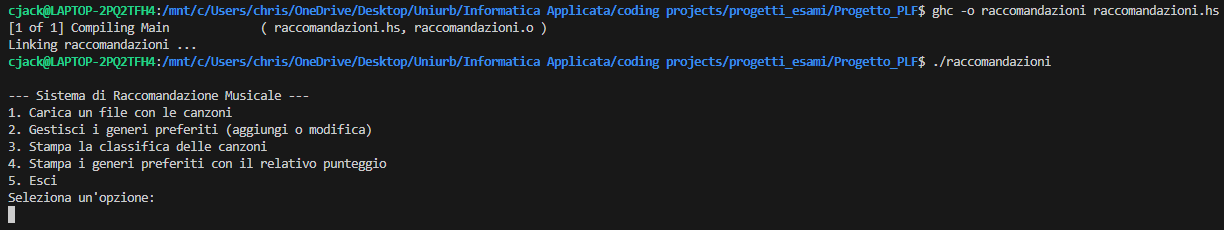
\includegraphics[width=0.8\textwidth]{Immagini/Tests/htest1.png}
    \end{center}
    \begin{center}
        \textbf{Test 2}
        \par
        \vspace{0.5cm}
        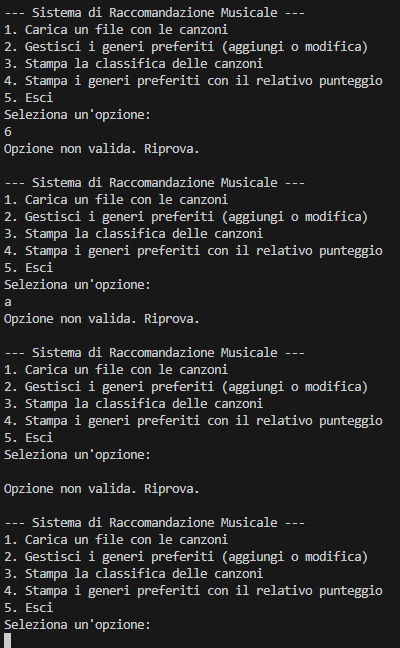
\includegraphics[width=0.6\textwidth]{Immagini/Tests/htest2}
    \end{center}
    \begin{center}
        \textbf{Test 3}
        \par
        \vspace{0.5cm}
        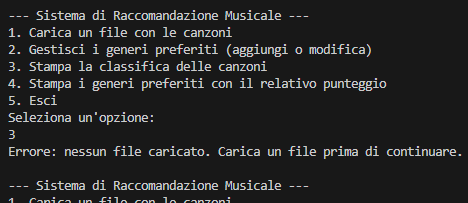
\includegraphics[width=1.0\textwidth]{Immagini/Tests/htest3}
    \end{center}
    \begin{center}
        \textbf{Test 4}
        \par
        \vspace{0.5cm}
        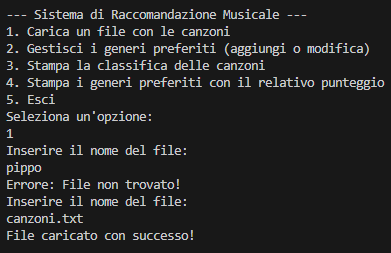
\includegraphics[width=0.8\textwidth]{Immagini/Tests/htest4}
    \end{center}

    \newpage
    \begin{center}
        \textbf{Test 5}
        \par
        \vspace{0.5cm}
        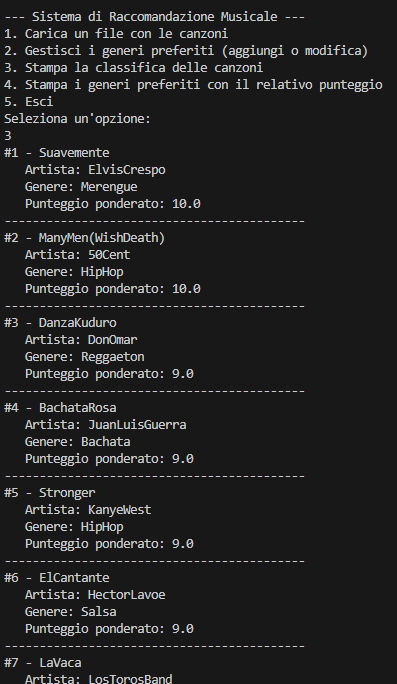
\includegraphics[width=1\textwidth]{Immagini/Tests/htest5}
    \end{center}
    \begin{center}
        \textbf{Test 6}
        \par
        \vspace{0.5cm}
        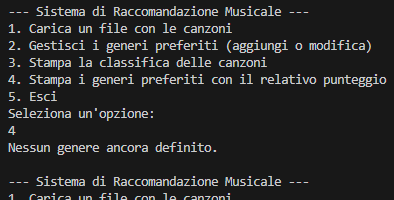
\includegraphics[width=1\textwidth]{Immagini/Tests/htest6}
    \end{center}

    \newpage
    \begin{center}
        \textbf{Test 7}
        \par
        \vspace{0.5cm}
        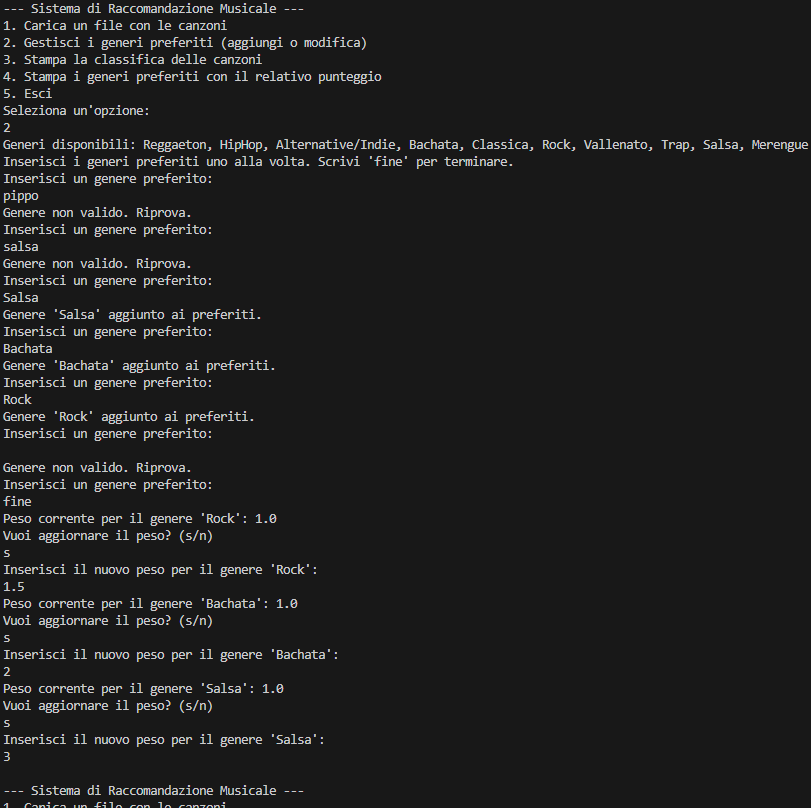
\includegraphics[width=1\textwidth]{Immagini/Tests/htest7}
    \end{center}
    \begin{center}
        \textbf{Test 8}
        \par
        \vspace{0.5cm}
        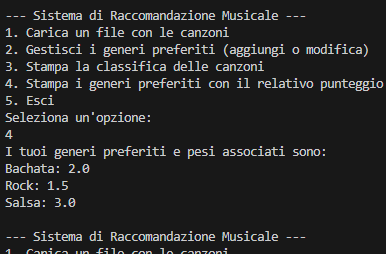
\includegraphics[width=1\textwidth]{Immagini/Tests/htest8}
    \end{center}

    \newpage
    \begin{center}
        \textbf{Test 9}
        \par
        \vspace{0.5cm}
        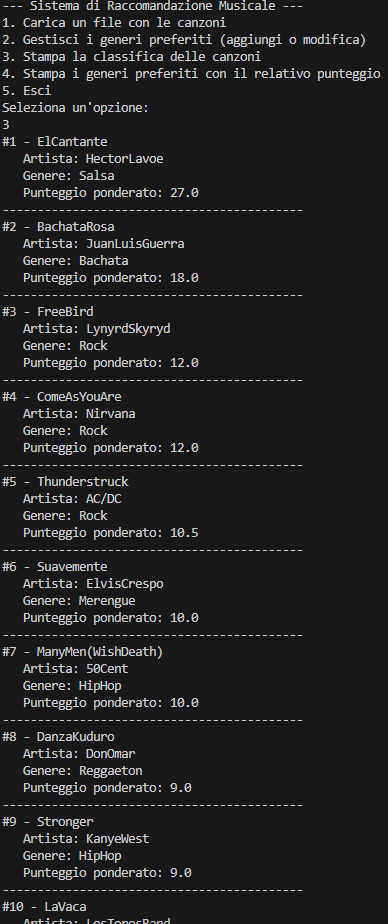
\includegraphics[width=1\textwidth]{Immagini/Tests/htest9}
    \end{center}
    \begin{center}
        \textbf{Test 10}
        \par
        \vspace{0.5cm}
        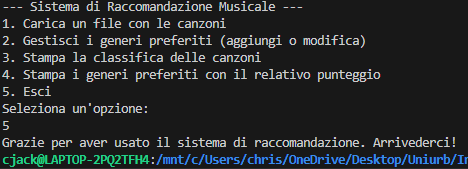
\includegraphics[width=1\textwidth]{Immagini/Tests/htest10}
    \end{center}
    \vspace{1cm}

    \newpage
    \subsection{Testing del programma in Prolog}
    \begin{center}
        \textbf{Test 1}
        \par
        \vspace{0.5cm}
        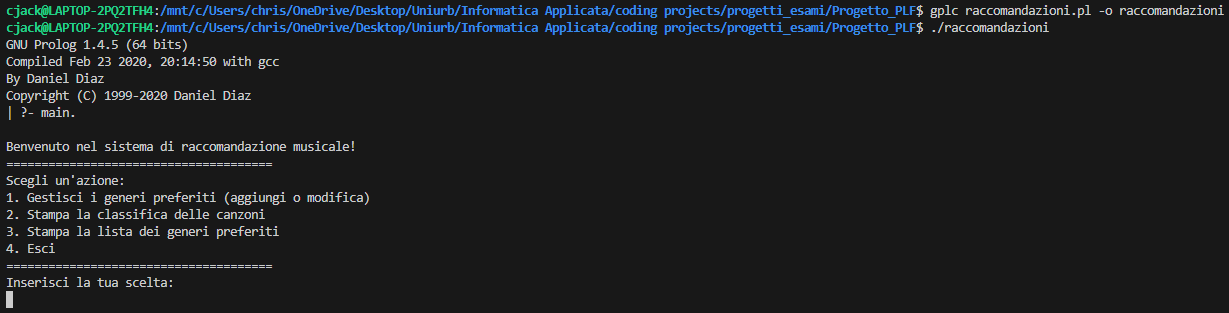
\includegraphics[width=1\textwidth]{Immagini/Tests/ptest1}
    \end{center}
    \begin{center}
        \textbf{Test 2}
        \par
        \vspace{0.5cm}
        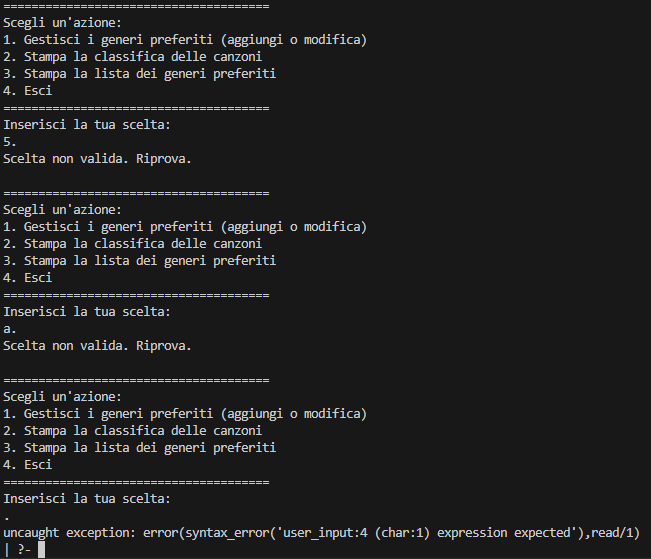
\includegraphics[width=1\textwidth]{Immagini/Tests/ptest2}
    \end{center}
    \begin{center}
        \textbf{Test 3}
        \par
        \vspace{0.5cm}
        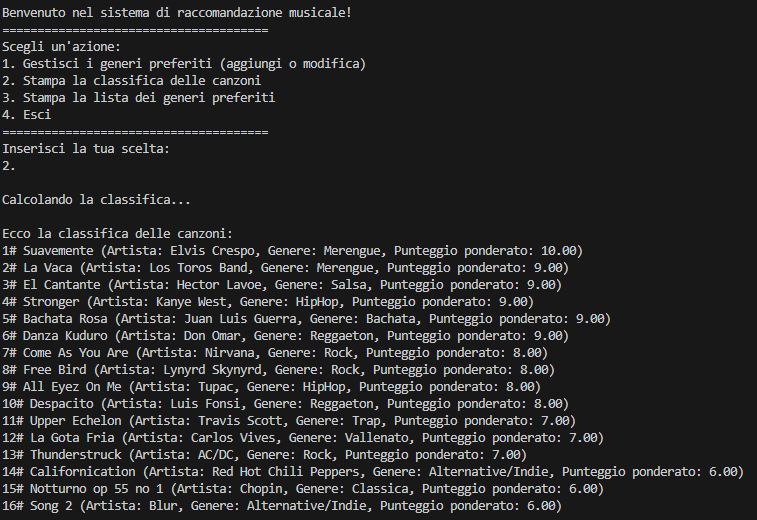
\includegraphics[width=1\textwidth]{Immagini/Tests/ptest3}
    \end{center}

    \newpage
    \begin{center}
        \textbf{Test 4}
        \par
        \vspace{0.5cm}
        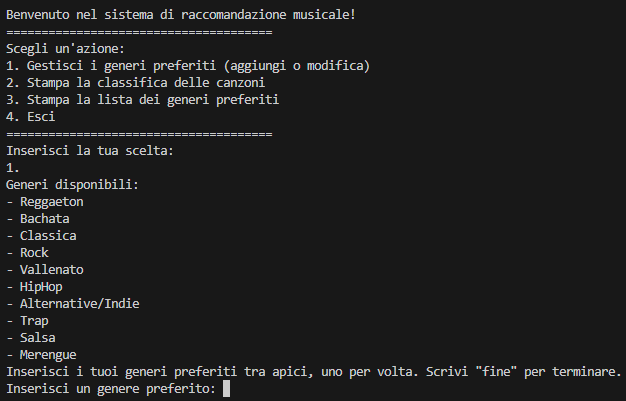
\includegraphics[width=1\textwidth]{Immagini/Tests/ptest4}
    \end{center}
    \begin{center}
        \textbf{Test 5}
        \par
        \vspace{0.5cm}
        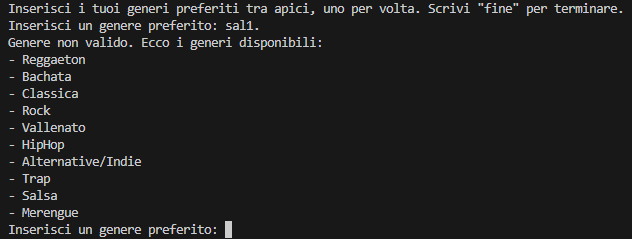
\includegraphics[width=1\textwidth]{Immagini/Tests/ptest5}
    \end{center}
    \begin{center}
        \textbf{Test 6}
        \par
        \vspace{0.5cm}
        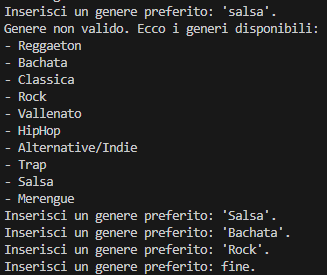
\includegraphics[width=1\textwidth]{Immagini/Tests/ptest6}
    \end{center}
    \begin{center}
        \textbf{Test 7}
        \par
        \vspace{0.5cm}
        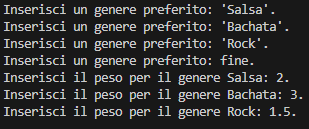
\includegraphics[width=1\textwidth]{Immagini/Tests/ptest7}
    \end{center}

    \newpage
    \begin{center}
        \textbf{Test 8}
        \par
        \vspace{0.5cm}
        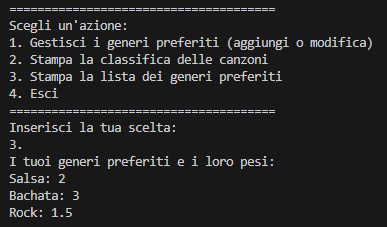
\includegraphics[width=1\textwidth]{Immagini/Tests/ptest8}
    \end{center}
    \begin{center}
        \textbf{Test 9}
        \par
        \vspace{0.5cm}
        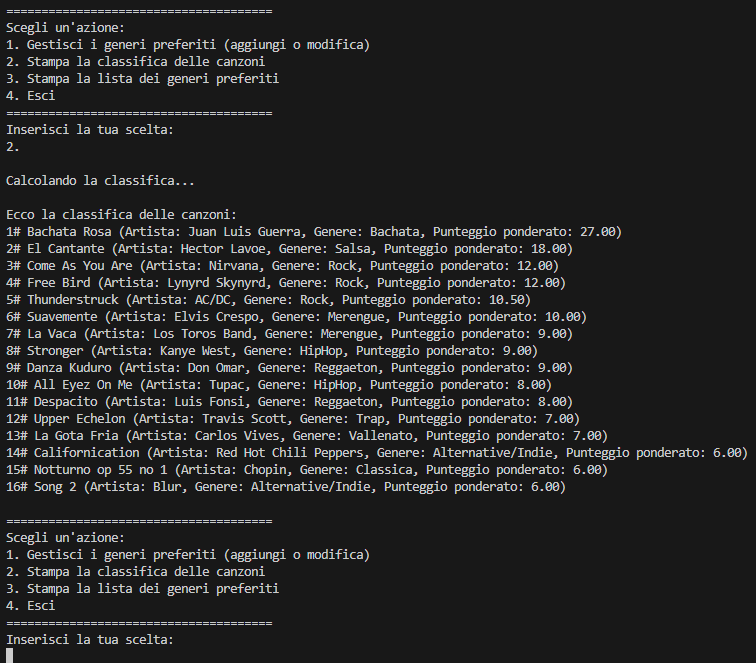
\includegraphics[width=1\textwidth]{Immagini/Tests/ptest9}
    \end{center}
    \begin{center}
        \textbf{Test 10}
        \par
        \vspace{0.5cm}
        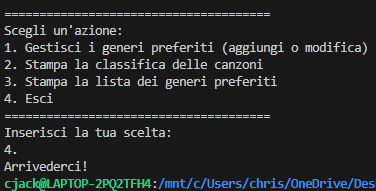
\includegraphics[width=1\textwidth]{Immagini/Tests/ptest10}
    \end{center}
    \vspace{1cm}

\end{document}